The corpus was assembled as a working library rather than a sample. It holds
\NBooks{} works by \NAuthors{} identified authors, printed between \YearMin{}
and \YearMax{}, and reaches the index in two forms: \NOcr{} passages were read
off page scans by OCR, and \NTxt{} came from typed editions. A passage is a
text block with a page and, for scanned material, a bounding box, so any
sentence quoted by the system can be traced back to a rectangle on an image.

It is not an even collection, and no analysis here pretends otherwise. The
median work contributes \MedianPassagesPerBook{} passages and the largest
contributes \MaxPassagesPerBook{}; a handful of multi-volume editions
therefore weigh as much as dozens of pamphlets. Figure~\ref{fig:corpus} shows
the distribution across time and the mix of the two text sources.

\begin{figure}[t]
  \centering
  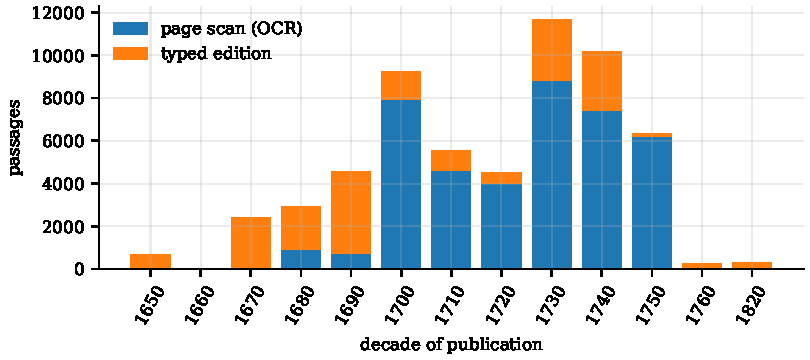
\includegraphics[width=\linewidth]{corpus_time.pdf}
  \caption{The corpus by decade of publication, split by how the text was
           obtained. The collection thickens sharply after 1700 and is
           dominated by scanned material; the typed editions are concentrated
           in the earlier period, where modern scholarly editions of women
           writers have been produced.}
  \label{fig:corpus}
\end{figure}

Two properties make the collection unusual and worth saying plainly. First,
its coverage of women writing moral philosophy is far heavier than a
conventional reading list: \WomenAuthors{} women contribute \WomenBooks{}
works and \WomenPassages{} passages, against \MenAuthors{} men with
\MenBooks{} works and \MenPassages{} passages. Second, the canonical figures
are present but not privileged; the index contains large quantities of
Rutherforth, Turnbull, Balfour and Campbell alongside Hutcheson and Hume.

Three services sit on top of the text and are used directly in what follows.
A lexical index serves BM25 \citep{robertson2009} over the OCR. A semantic
index holds every passage as a 2048-dimensional vector produced by a
sentence-transformer \citep{reimers2019}, searched by cosine on a GPU. A
retrieval agent, served by vLLM \citep{kwon2023}, calls both along with a
page-level reader, and is the component that turns a question into cited
passages. The analyses below call the same running endpoints the website
calls, so what is measured is the deployed system and not a reimplementation
of it.
